\documentclass{article}

\usepackage[a4paper]{geometry}
\usepackage[ngerman]{babel}
\usepackage[utf8]{inputenc}
\usepackage[T1]{fontenc}
\usepackage{graphicx}
\usepackage{fancyhdr}
\usepackage{xcolor}
\usepackage{float}
\usepackage{hyperref}
\usepackage{url}
\graphicspath{{./images/}}

\pagestyle{fancyplain}
\fancyhf{}
\lhead{\fancyplain{}{Gruppe 11 – Mathias Baumbach \& Mara Schulke}}
\rhead{\fancyplain{}{\today}}
\cfoot{\fancyplain{}{\thepage}}

\begin{document}

\begin{titlepage}
	\begin{flushleft}
		TH Brandenburg \\
		Online Studiengang IT Sicherheit \\
		Fachbereich Informatik und Medien \\
		Netzwerksicherheit \\
		Prof.\ Dr.\ Michael Pilgermann
	\end{flushleft}

	\vfill

	\begin{center}
		\Large{Zusatz-Einsendeaufgabe 1}\\[0.5em]
		\large{Wintersemester 2023}\\[0.25em]
		\large{\today}
	\end{center}

	\vfill

	\begin{flushright}
		Gruppe 11 \\
		Mathias Baumbach (Matr-Nr. 20213703) \\
		Mara Schulke (Matr-Nr. 20215853)
	\end{flushright}
\end{titlepage}

\begin{abstract}
\end{abstract}

\tableofcontents

\listoffigures

\newpage

\section{Introduction}

Firewalls are one of the basic, yet very effective security controls in network 
security. Packet filters is the entry level firewall technology.

The experiment shall secure a topology with three network segments, which are each 
connected to a unique port at a firewall:

\begin{itemize}
    \item Client-LAN: Client network (1 admin client, 1 user client; both Ubuntu Linux)
    \item Server-LAN: Server network (1 server acting as web server; Ubuntu Server)
    \item WAN: External network
\end{itemize}

\begin{figure}[H]
	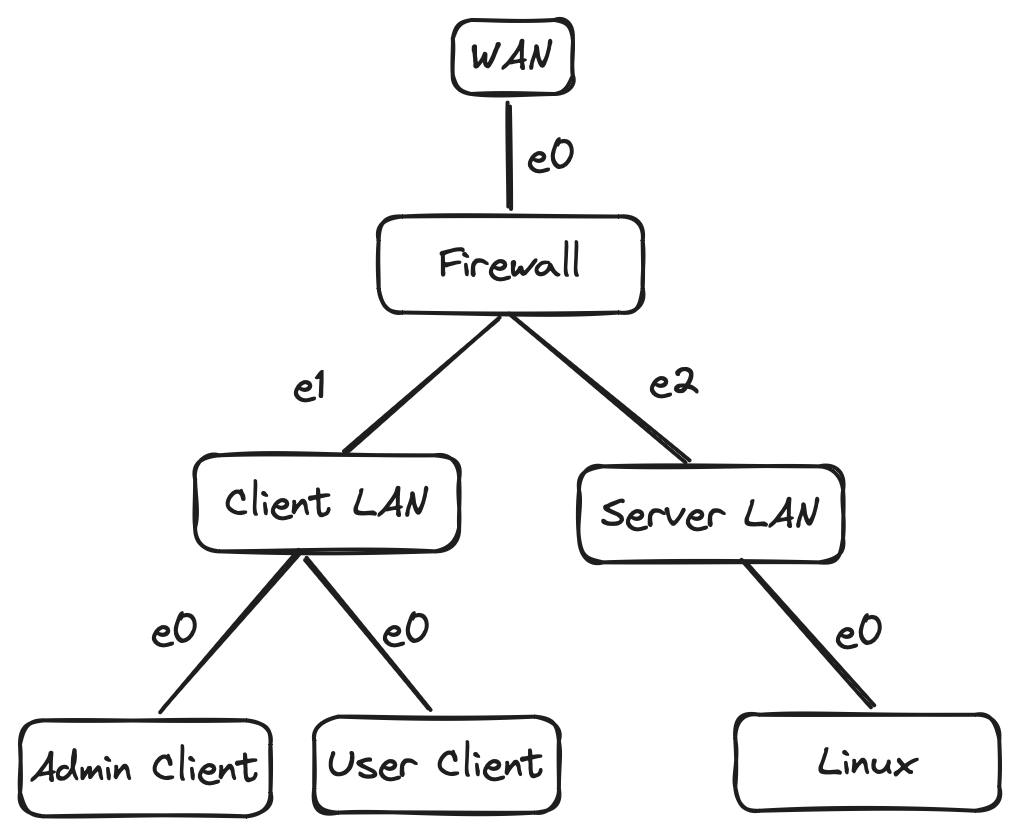
\includegraphics[width=0.75\textwidth]{images/01}
	\centering
	\caption{Netztopologie}
\end{figure}

The topology with the firewall (pfSense), three Ubuntu boxes (2 clients and one 
server) and the external connection has been prepared in the virtual lab environment 
already. However, the ruleset of the firewall is empty; the exercise is about 
developing a ruleset based on the “white listing” paradigm, implementing it on the 
firewall and checking connectivity.

The following communication shall be allowed (including corresponding reply traffic):

\begin{itemize}
    \item All endpoints (server as well as clients) shall connect to the external net for HTTP / HTTPS traffic on the corresponding ports.
    \item The admin client shall connect to the server via SSH.
\end{itemize}

\section{Preparation}

\subsection{Connect to lab (VNL) and initialize systems}

Connect to the Virtual Network Security Lab (VNL) of THB using your web browser as 
documented (incl. group credentials). 

Navigate to shared space in VNL and create a copy of the lab \path{Shared/
Netzwerksicherheit/2023_exercise_firewalls.unl}\\
and place the copy in your user folder. Boot up the systems in your lab – make sure, 
to always start with the pfSense-Firewall, as this one acts as DHCP-Server for the 
clients and the server. When booting the systems for the first time, some initial 
configuration has to be applied – check \textbf{appendix 1 – startup configurations} 
at the end of this document for details. 

\subsection{Check communication between components}

Open up the user interface for each component (command line for servers, remote 
desktop for clients) inside your web browser; login using the eve-ng default 
credentials. 

Check connectivity internally (web server via IP) and to the outside world (e.g. web 
browser on GUI environments or wget on command line). Document your network topology 
in a corresponding plan including the IP addresses. 

\subsubsection*{Antwort}

Zur Dokumentation der Netztopologie haben wir unsere grafische Darstellung der 
Netzwerktopologie um die IP Adressen erweitert:

\begin{figure}[H]
	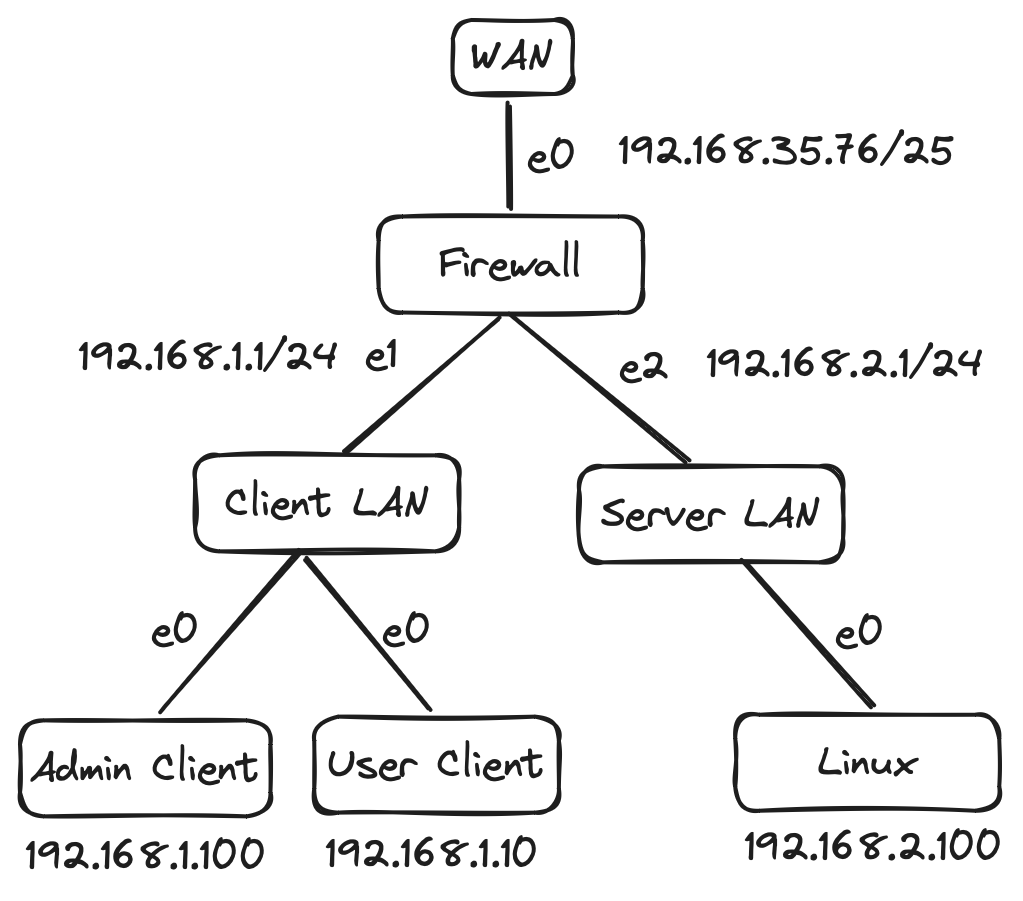
\includegraphics[width=0.75\textwidth]{images/02}
	\centering
	\caption{Dokumentierte Netztopologie mit IP-Adressen}
\end{figure}

\vspace{0.5em}

\subsection{Access your group firewall}

Using the remote desktop of the admin client, open firewall web gui in the web 
browser. Get a very first impression of the ruleset and familiarize yourself with the 
handling.

\section{Execution}

Having tested, that the lab environment works fine including all communication, next 
action is to step-by-step restrict the firewall ruleset.

\subsection{Part 1: Effective firewall rules}

Prepare a table for documentation of your firewall policy. Include at least: Type 
(l4), source IP, source port, destination IP, destination port, action. This policy / 
documentation shall always be updated before applying changes to the firewall 
ruleset.

\subsubsection*{Antwort}

\vspace{5mm}

Unsere Tabelle der pfSense Firewall Policies ist bereits mit einigen Standard-Regeln, 
die pfSense initial anlegt, gefüllt:

\begin{center}
    %ghetto fix um table auf page zu bekommen 
    \resizebox{\textwidth}{!}{\begin{tabular}{||c c c c c c c c||} 
         \hline
            VLAN    & Type (I4)  & Source IP  & Source Port & Destination IP& Destination Port & Action & Beschreibung  \\ [0.3ex] 
         \hline\hline
            LAN  & Any   & Any  & Any  & LAN Address   & 443 \& 80  & allow  & Anti-Lockout Rule  \\ 
         \hline
            LAN & Any & EasyRuleBlock HostVLAN   & Any  & Any  & Any & block & Durch initiale Configuration angelegt  \\ 
         \hline
            LAN & IPv4/IPv6 & LAN & Any  & Any  & Any & allow & Default allow LAN to any rule  \\ 
         \hline
            SERVER\_LAN & IPv4/IPv6 & SERVER\_LAN & Any  & Any  & Any & allow & Default allow SERVER\_LAN to any rule  \\ 
         \hline
    \end{tabular}}
\end{center}


\subsubsection{Implement white listing for outgoing traffic}

The default behavior of the firewall for outgoing traffic (“black listing”) shall be 
inversed. This is achieved by changing the default rule. The default rule of a 
ruleset will always apply, if no other rule matched the traffic before. The 
configuration needs to be applied to the 2 LAN interfaces. 

\subsubsection*{Antwort}

Die default deny Regeln im pfSense Menü:

\begin{figure}[H]
	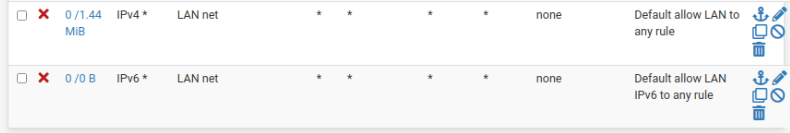
\includegraphics[width=0.75\textwidth]{images/03}
	\centering
	\caption{Lan VLAN Default Rule}
\end{figure}

\begin{figure}[H]
	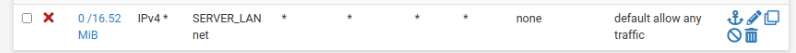
\includegraphics[width=0.75\textwidth]{images/04}
	\centering
	\caption{Server\_LAN VLAN Default Rule}
\end{figure}

Unsere Tabelle der pfSense Firewall Policies mit den veränderten default Regeln:

\begin{center}
    %ghetto fix um table auf page zu bekommen 
    \resizebox{\textwidth}{!}{\begin{tabular}{||c c c c c c c c||} 
         \hline
            VLAN & Type (I4)  & Source IP  & Source Port & Destination IP& Destination Port & Action & Beschreibung\\ [0.3ex] 
         \hline\hline
            LAN & Any & Any  & Any  & LAN Address & 443 \& 80  & allow  & Anti-Lockout Rule\\ 
         \hline
            LAN & Any & EasyRuleBlock HostVLAN & Any  & Any  & Any & block & Durch initiale Konfiguration angelegt\\ 
         \hline
            LAN & IPv4/IPv6 & LAN & Any  & Any  & Any & deny & Default deny LAN to any rule\\ 
         \hline
            SERVER\_LAN & IPv4/IPv6 & SERVER\_LAN & Any  & Any  & Any & deny & Default deny SERVER\_LAN to any rule\\ 
         \hline
    \end{tabular}}
\end{center}



\subsubsection{Allow for http/https traffic}

Add additional rules for allowing http/https traffic from all clients / servers. 
Which ports are required? TCP or UDP? Adopt your firewall policy before applying 
changes to the firewall.

Test your firewall configuration by web browsing from within your ubuntu client. 

\subsubsection*{Antwort}

Bevor man den Datenverkehr auf Port 80 \& 443 erlaubt für http/https, erhält man die 
folgende Meldung beim Aufruf unseres Webservers:

\begin{figure}[H]
	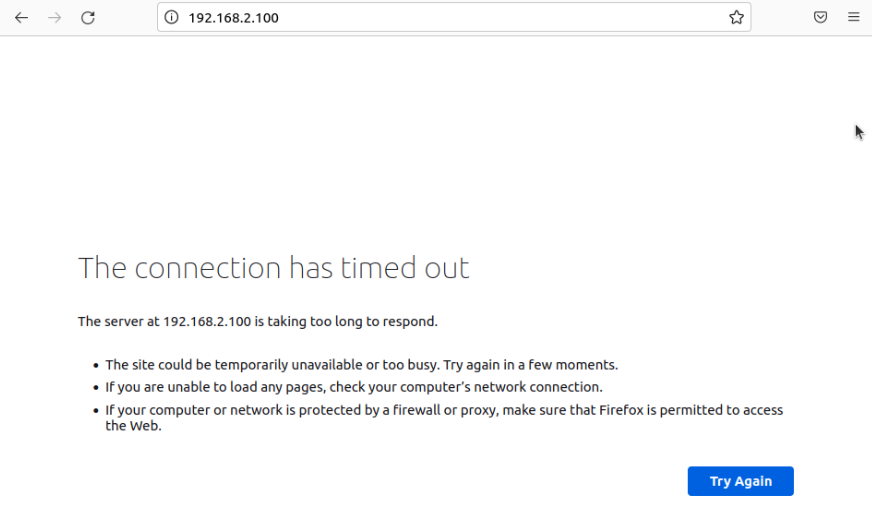
\includegraphics[width=0.75\textwidth]{images/05}
	\centering
	\caption{Fehlgeschlagener Aufruf des Webservers via IP-Adresse}
\end{figure}

Um diese Fehlermeldung zu umgehen sind folgende zusätzliche Firewall Regeln nötig:

\begin{center}
    %ghetto fix um table auf page zu bekommen 
    \resizebox{\textwidth}{!}{\begin{tabular}{||c c c c c c c||} 
         \hline
            VLAN & Type (I4)  & Source IP  & Source Port & Destination IP& Destination Port & Action \\ [0.3ex] 
         \hline\hline
            LAN & TCP & LAN net VLAN & Any & Any & 80 (http) & allow\\ 
         \hline
            LAN & TCP & LAN net VLAN & Any & Any & 443 (https) & allow\\ 
         \hline
            SERVER\_LAN & TCP & SERVER\_LAN net VLAN & Any & Any & 80 (http) & allow\\ 
         \hline
            SERVER\_LAN & TCP & SERVER\_LAN net VLAN & Any & Any & 443 (https) & allow\\ 
         \hline
    \end{tabular}}
\end{center}

Nun kann bei erneutem Aufruf der IP unseres Webservers erfolgreich die Webseite 
abgerufen werden:

\begin{figure}[H]
	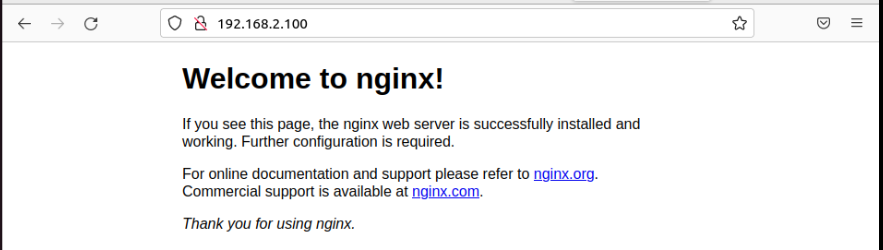
\includegraphics[width=0.75\textwidth]{images/06}
	\centering
	\caption{Erfolgreicher Aufruf des Webservers via IP-Adresse}
\end{figure}

\subsubsection{Which additional traffic is required?}

You should experience issues when browsing the web. 

Discuss: Which additional traffic is required? Which changes need to be applied to 
your firewall policy? Adopt and test again. 

\subsubsection*{Antwort}

Unser Webserver war in der vorherigen Aufgabe erreichbar, weil der Aufruf per IP-
Adresse erfolgte. Für Zugriff auf Webseiten im Internet ist die Anfrage an einen DNS 
Server nötig, der die URL in eine IP Adresse für den Browser übersetzt.

Da wir bisher keine Regel für DNS Traffic angelegt haben, schlägt ein Aufruf einer 
URL fehl:

\begin{figure}[H]
	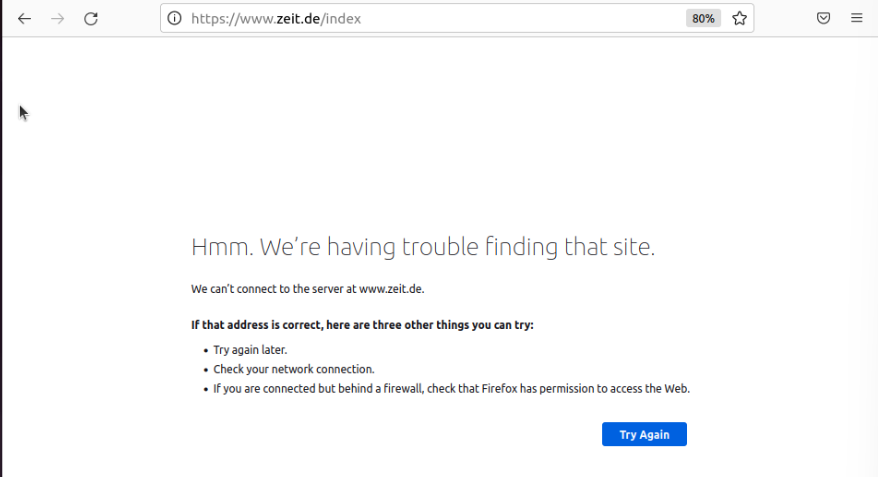
\includegraphics[width=0.75\textwidth]{images/07}
	\centering
	\caption{Fehlgeschlagener Aufruf eines Webservers via URL}
\end{figure}

Es sind folgende zusätzliche Firewall Regeln nötig:

\begin{center}
    %ghetto fix um table auf page zu bekommen 
    \resizebox{\textwidth}{!}{\begin{tabular}{||c c c c c c c||} 
         \hline
            VLAN    & Type (I4)  & Source IP  & Source Port & Destination IP& Destination Port & Action \\ [0.3ex] 
         \hline\hline
            LAN  & TCP/UDP   & LAN net VLAN & Any  & Any   & 53 (dns)  & allow  \\ 
         \hline
            SERVER\_LAN  & TCP/UDP & LAN net VLAN  & Any  & Any   & 53 (dns)  & allow  \\ 
         \hline
    \end{tabular}}
\end{center}

Dadurch können nun Webseiten-Aufrufe im Internet erfolgreich übersetzt werden: 

\begin{figure}[H]
	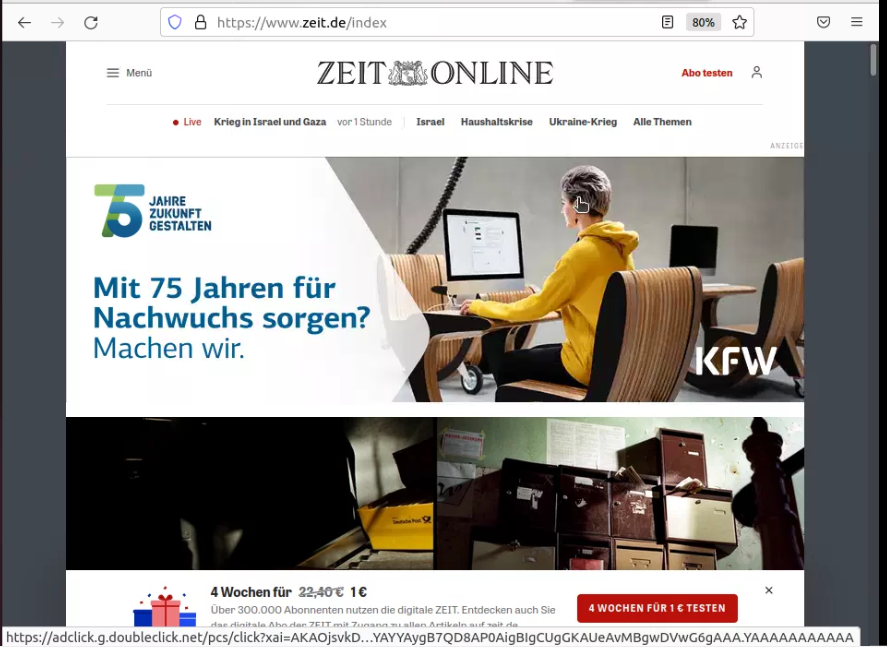
\includegraphics[width=0.75\textwidth]{images/08}
	\centering
	\caption{Erfolgreicher Aufruf eines Webservers via URL}
\end{figure}

Darüber hinaus gäbe es noch weitere Ports, deren Freigabe nützlich wäre. Beispiel 
wären WebRTC (Port-Range 48k bis 65k?) oder IMAP (143).  

\subsubsection{Secure admin access}

SSH access to the server should be restricted to the admin client; all other traffic 
between those two networks shall be prohibited. 

\begin{itemize}
    \item Add a rule for allowing access to the webserver (HTTP / HTTPS) from any endpoint in the client LAN. 
    \item Add a rule for allowing admin access to the webserver (SSH) from the admin client. 
\end{itemize}

Test the communication. 

\subsubsection*{Antwort}

Die default deny Regel verhindert den SSH Zugang vom Admin- und vom User-Client zum Server:

\begin{figure}[H]
	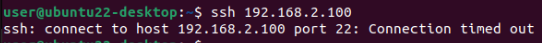
\includegraphics[width=0.75\textwidth]{images/09}
	\centering
	\caption{SSH Verbindung vom Admin-Client zum Server}
\end{figure}

\begin{figure}[H]
	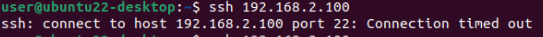
\includegraphics[width=0.75\textwidth]{images/10}
	\centering
	\caption{SSH Verbindung vom User-Client zum Server}
\end{figure}

Es ist folgende zusätzliche Firewall Regeln nötig:

\begin{center}
    %ghetto fix um table auf page zu bekommen 
    \resizebox{\textwidth}{!}{\begin{tabular}{||c c c c c c c||} 
         \hline
            VLAN    & Type (I4)  & Source IP  & Source Port & Destination IP& Destination Port & Action \\ [0.3ex] 
         \hline\hline
            LAN  & TCP   & 192.168.1.100 & Any  & SERVER\_LAN net VLAN  & 22 (SSH)  & allow  \\ 
         \hline
    \end{tabular}}
\end{center}

Nach Aktivierung dieser Regel ist der SSH Zugriff weiterhin für den User-Client 
geblockt, für den Admin-Client aber möglich:

\begin{figure}[H]
	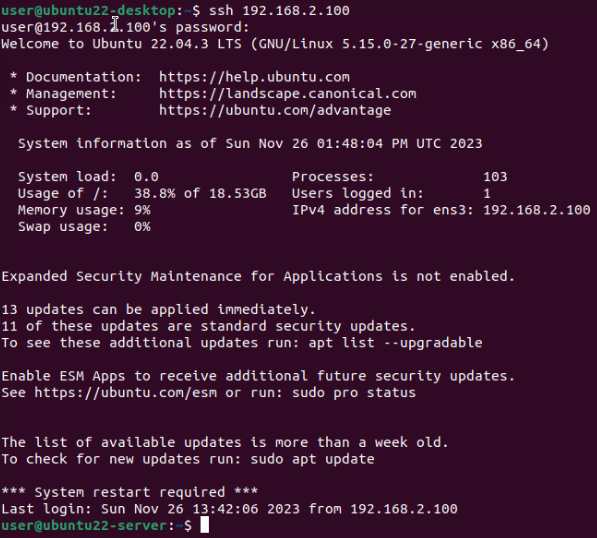
\includegraphics[width=0.75\textwidth]{images/11}
	\centering
	\caption{SSH Verbindung vom Admin-Client zum Server mit SSH Regel}
\end{figure}

\begin{figure}[H]
	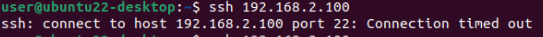
\includegraphics[width=0.75\textwidth]{images/12}
	\centering
	\caption{SSH Verbindung vom User-Client zum Server mit SSH Regel}
\end{figure}


\subsection{Part 2: Analyze firewall audit trail}

Apply changes to your firewall ruleset, so that events are being logged whenever 
anybody accesses the server on port 22 (no matter whether it is successful or not). 

Trigger those firewall rules by starting SSH connection to the serves from 

\begin{itemize}
    \item 1) the admin client and 
    \item 2) the “normal” client. 
\end{itemize}

Observe the events in the audit trail on the firewall. 

\subsubsection*{Antwort}

Für diese Aufgabe müssen zwei Regeln aus den vorherigen Aufgaben erweitert werden:

\begin{center}
    %ghetto fix um table auf page zu bekommen 
    \resizebox{\textwidth}{!}{\begin{tabular}{||c c c c c c c||} 
         \hline
            VLAN & Type (I4) & Source IP & Source Port & Destination IP& Destination Port & Action \\ [0.3ex] 
         \hline\hline
            LAN & TCP & 192.168.1.100 & Any & SERVER\_LAN net VLAN & 22 (SSH) & allow\\ 
         \hline
            LAN & IPv4/IPv6 & LAN net VLAN & Any  & Any  & Any & deny\\ 
         \hline      
    \end{tabular}}
\end{center}

An beiden Regeln muss die Extra Option ''Log packets that are handled by this rule`` 
angehakt werden.

Danach kann in den System Logs der pfSense (Status / System Logs / Firewall / Dynamic 
View) der erfolgreiche und erfolglose ssh Verbindungsversuch verfolgt werden:

\begin{figure}[H]
	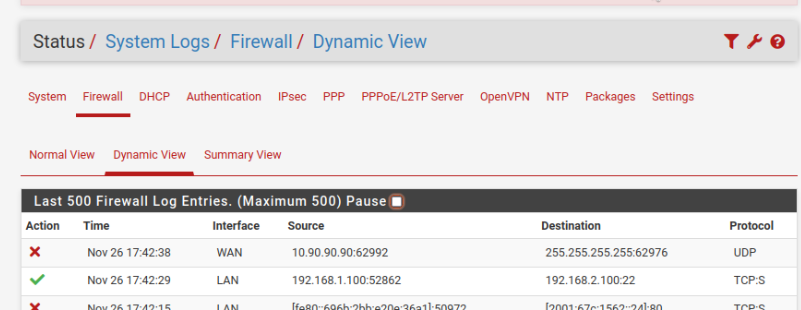
\includegraphics[width=0.75\textwidth]{images/13}
	\centering
	\caption{Erfolgreiche SSH Verbindung vom Admin-Client}
\end{figure}

In der 2. Zeile (grüner Haken) kann man den erfolgreichen Zugriff von 192.168.1.100 
Port 52862 auf 192.168.2.100 Port 22 beobachten.

\begin{figure}[H]
	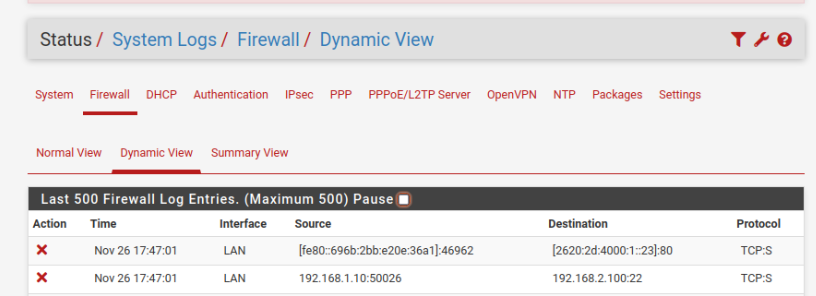
\includegraphics[width=0.75\textwidth]{images/14}
	\centering
	\caption{Erfolglose SSH Verbindung vom User-Client}
\end{figure}

Ebenfalls in der 2. Zeile ist der fehlgeschlagene Zugriff von 192.168.1.10 Port 50026 
auf 192.168.2.100 Port 22 dokumentiert.

\section{References / Documentation}

\begin{itemize}
    \item 1) Eve-ng cookbook: \path{https://www.eve-ng.net/index.php/documentation/professional-cookbook/} 
    \item 2) pfSense Firewall configuration documentation: \path{https://docs.netgate.com/pfSense/en/latest/firewall/index.html}
\end{itemize}

\end{document}